\section{System}
\label{sec:sys}

\begin{figure}[t!]
\begin{center}
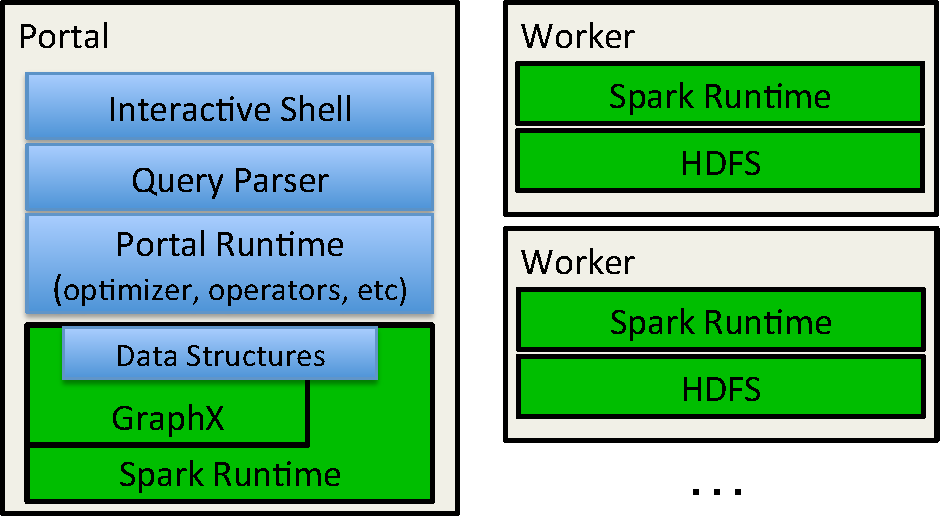
\includegraphics[height=1.4in]{figs/architecture.pdf}
\caption{\ql system architecture.}
\label{fig:arch}
\end{center}
\end{figure}

Our \ql system builds on GraphX, an Apache Spark library, as depicted
in Figure~\ref{fig:arch}.  Green boxes indicate built-in components,
while blue are those we added for \ql.  We selected Apache Spark
because it is a popular open-source system, and because of its
in-memory processing approach.  All language operators on evolving
graphs, \tg for short, are available through the public API of the \ql
library, and may be used like any other library in an Apache Spark
application.

\subsection{Language}
\label{sec:language}

The basic element of our system is a graph that evolves over time.  A
snapshot represents a single state of an evolving graph, and is not
time-aware.  Temporal evolution of a graph is represented by a
sequence of snapshots, called a {\em temporal graph}, or \tg for
short, with an associated temporal sequence.  A temporal sequence, in
turn, is a sequence of consecutive non-overlapping open-closed time
periods of the same duration.

The \ql query language is declarative.  We support unary and binary
operators that take \tgs as input and produce a \tg as output.  Thus,
the language is fully compositional.  \ql uses SQL-like syntax, and
has the form \insql{TSelect} \ldots \insql{From} \ldots \insql{TWhere}
\ldots \insql{TGroup}.  We prefix temporal keywords with \insql{T}, to
make the distinction between \ql and SQL operations explicit.  \ql
supports evolving graph-specific operations such as snapshot analytics
(e.g., pagerank) and temporal aggregation, along with generic
set-based operations such as a join.

For example, consider the following query:

\begin{small}
\begin{verbatim}
Q1:  TSelect Any V [vid, any(name), max(salary)] ; 
             Any E [vid1, vid2, sum(cnt)] 
     From T1 
     TGroup by 2 years
\end{verbatim}
\end{small}

\insql{Q1} temporally aggregates evolving graph T1 snapshots in 2 year
increments, followed by a projection ($max(salary)$ and $sum(cnt)$ are
parts of aggregation).  A more complex query using 5 operations:

\begin{small}
\begin{verbatim}
Q2:  TSelect Any V [vid, pagerank() as pr] ; 
             Any E [vid1, vid2] 
     From    T1 TAnd T2 
     TWhere  Start >= 2012 And End <= 2014 
     TGroup by 2 years
\end{verbatim}
\end{small}

\insql{Q2} uses temporal join ($TAnd$), followed by temporal selection
($TWhere$), aggregation ($TGroup$), snapshot analytics, and
projection.  For more detail about the language, please see~\cite{}.

\subsection{Query Processing}
\label{sec:queryp}

\begin{figure}
\begin{center}
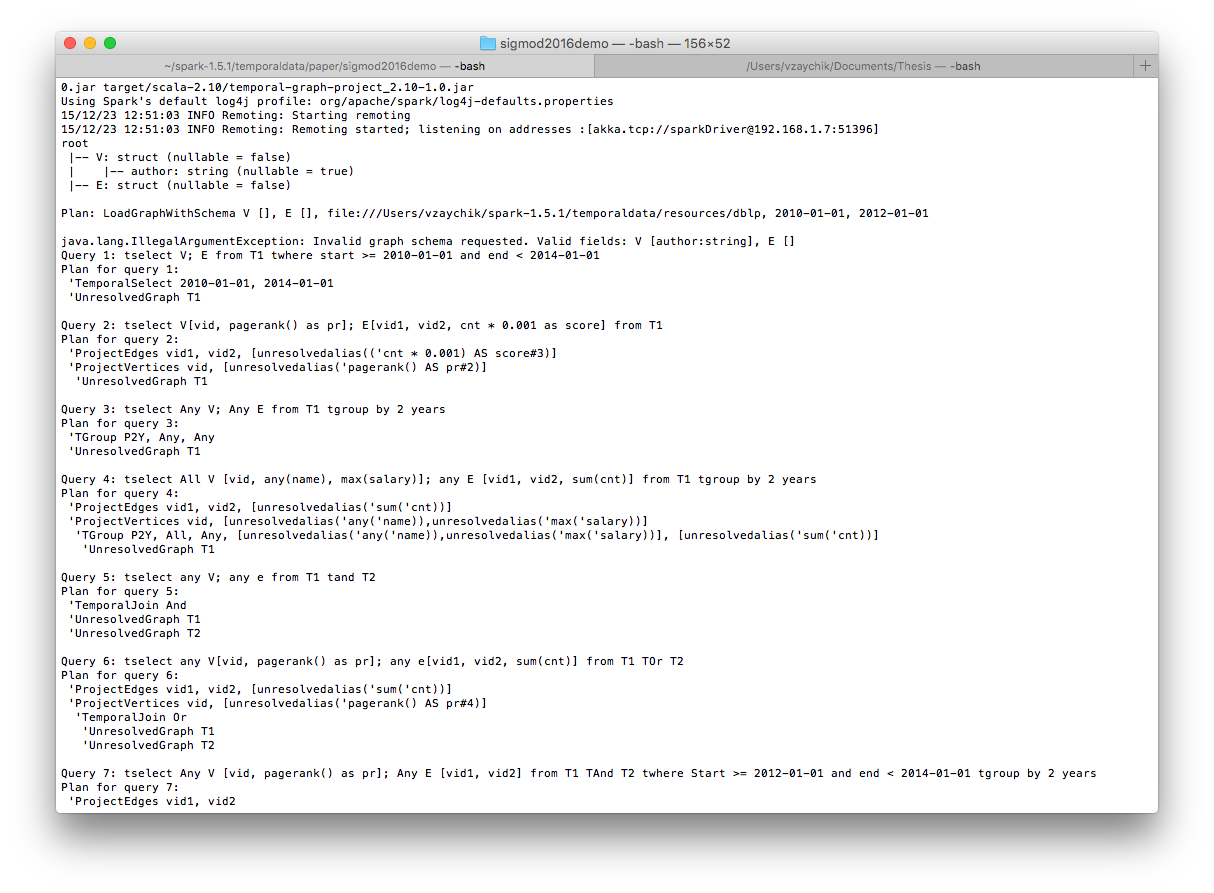
\includegraphics[width=3.2in]{figs/shell.png}
\caption{\ql shell session. PLACEHOLDER}
\label{fig:shell}
\end{center}
\end{figure}

The \ql system includes an interactive shell for exploratory data
analysis (Figure~\ref{fig:shell}).  \ql query execution follows the
traditional RDBMS query processing steps: parsing, logical plan
generation and verificaton, and physical plan generation.  \ql re-uses
and extends SparkSQL abstractions for these steps.  A \ql query is
rewritten into a sequence of operators, and some operators are
reordered to improve performance.  We developed several different
physical representations and partition strategies that are selected at
the physical plan generation stage.  The evolving graph snapshots are
read from the distributed file system HDFS and processed by Spark
Workers, with the tasks assigned and managed by the runtime.

Shell users can:
\begin{enumerate}[leftmargin=*]
\item Define materialized and unmaterialized views of \tg using
  standard SQL \insql{define view} command.
\item View logical plans for defined views using \insql{describe}
  command.
\item View results of queries using SQL, with \ql queries either
  embedded in SQL or from a previously defined view.
\item View defined views and functions, including snapshot analytics.
\end{enumerate}

The SQL query below shows \insql{vid} and \insql{tr} values of 20
vertices with the most significantly increasing \insql{pagerank}
trend.

\begin{small}
\begin{verbatim}
Q3:   Select   VF.vid, VF.tr  
      From     T5.toVerticesFlat() as VF
      Order by tr
      Limit    20
\end{verbatim}
\end{small}

The important part of \insql{Q3} is the use of
\insql{T5.toVerticesFlat()} in the \insql{From} clause.  This is an
operation provided by the \ql framework, which collects all vertices
in the union of snapshots of \insql{T5} into a single nested vertex
collection and flattens it into \insql{VF} (\underline{vid}:int,
\underline{start}:date, \underline{end}:date, tr:float, mx:float).
\insql{VF} can be used in SQL queries.  \ql also provides an operation
that returns a flattened collection of edges, called
\insql{toEdgesFlat()}.
